With the development of algorithms and hardware platforms, Convolutional Neural Network (CNN) has greatly improved the perception and decision-making ability of unmanned platform. 
% such as object detection \cite{redmon2018yolov3} and scene segmentation \cite{huang2019mask} in perception, and path planning \cite{chen2017socially} and dynamic obstacle avoidance \cite{kaufmann2018deep} in decision-making.

Distributed Simultaneously Localization and Mapping (DSLAM) is a basic task for many multi-robot applications, and is a hot topic in robotics. There are two key modules which consume most of the computation: Feature-point Extraction (FE) and Place Recognition (PR). 
FE provides the feature-points for the Visual Odometry (VO) to calculate the relative pose between two adjacent frames. PR generates the compact image representation, which produces the candidate place recognition matches between different robots. 
Recent works use CNN to extract feature-points  ~\cite{detone2018superpoint, simo2015discriminative, yi2016lift} and generate the place representation code  ~\cite{arandjelovic2016netvlad, radenovic2018fine}. 
The CNN-based feature-point extraction method, SuperPoint  ~\cite{detone2018superpoint}, achieves 10\%-30\% higher matching accuracy compared with the popular handcrafted extraction method, ORB ~\cite{Mur-Artal:2017281}.
The accuracy of the place recognition code from another CNN-based method, GeM  ~\cite{radenovic2018fine}, is also about 20\% better than the handcrafted method, rootSIFT  ~\cite{jegou2014triang}.

However, CNN is computation consuming. A single inference forward of the CNN-based SuperPoint feature-point extraction consumes 39G operations  ~\cite{detone2018superpoint}, and a single inference forward of the CNN-based GeM  place recognition consumes 192G operations  ~\cite{radenovic2018fine}.
Thus, specific hardware architectures on FPGA  ~\cite{guo2017angel,yu2018instruction,li_high_2016,qiu2016going,lu_evaluating_2017} are designed to deploy CNN on the embedded system.
With the help of network quantization and on-chip data reuse, the speed of CNN accelerators on embedded FPGA achieves 3TOP/s  ~\cite{lu_evaluating_2017}, which can support the real-time execution of CNN-based feature-point extraction  ~\cite{detone2018superpoint}.
However, these CNN accelerators are designed and optimized to accelerate a single CNN. They can not automatically schedule two or more tasks simultaneously. 


\begin{figure}[t]
	\centering
    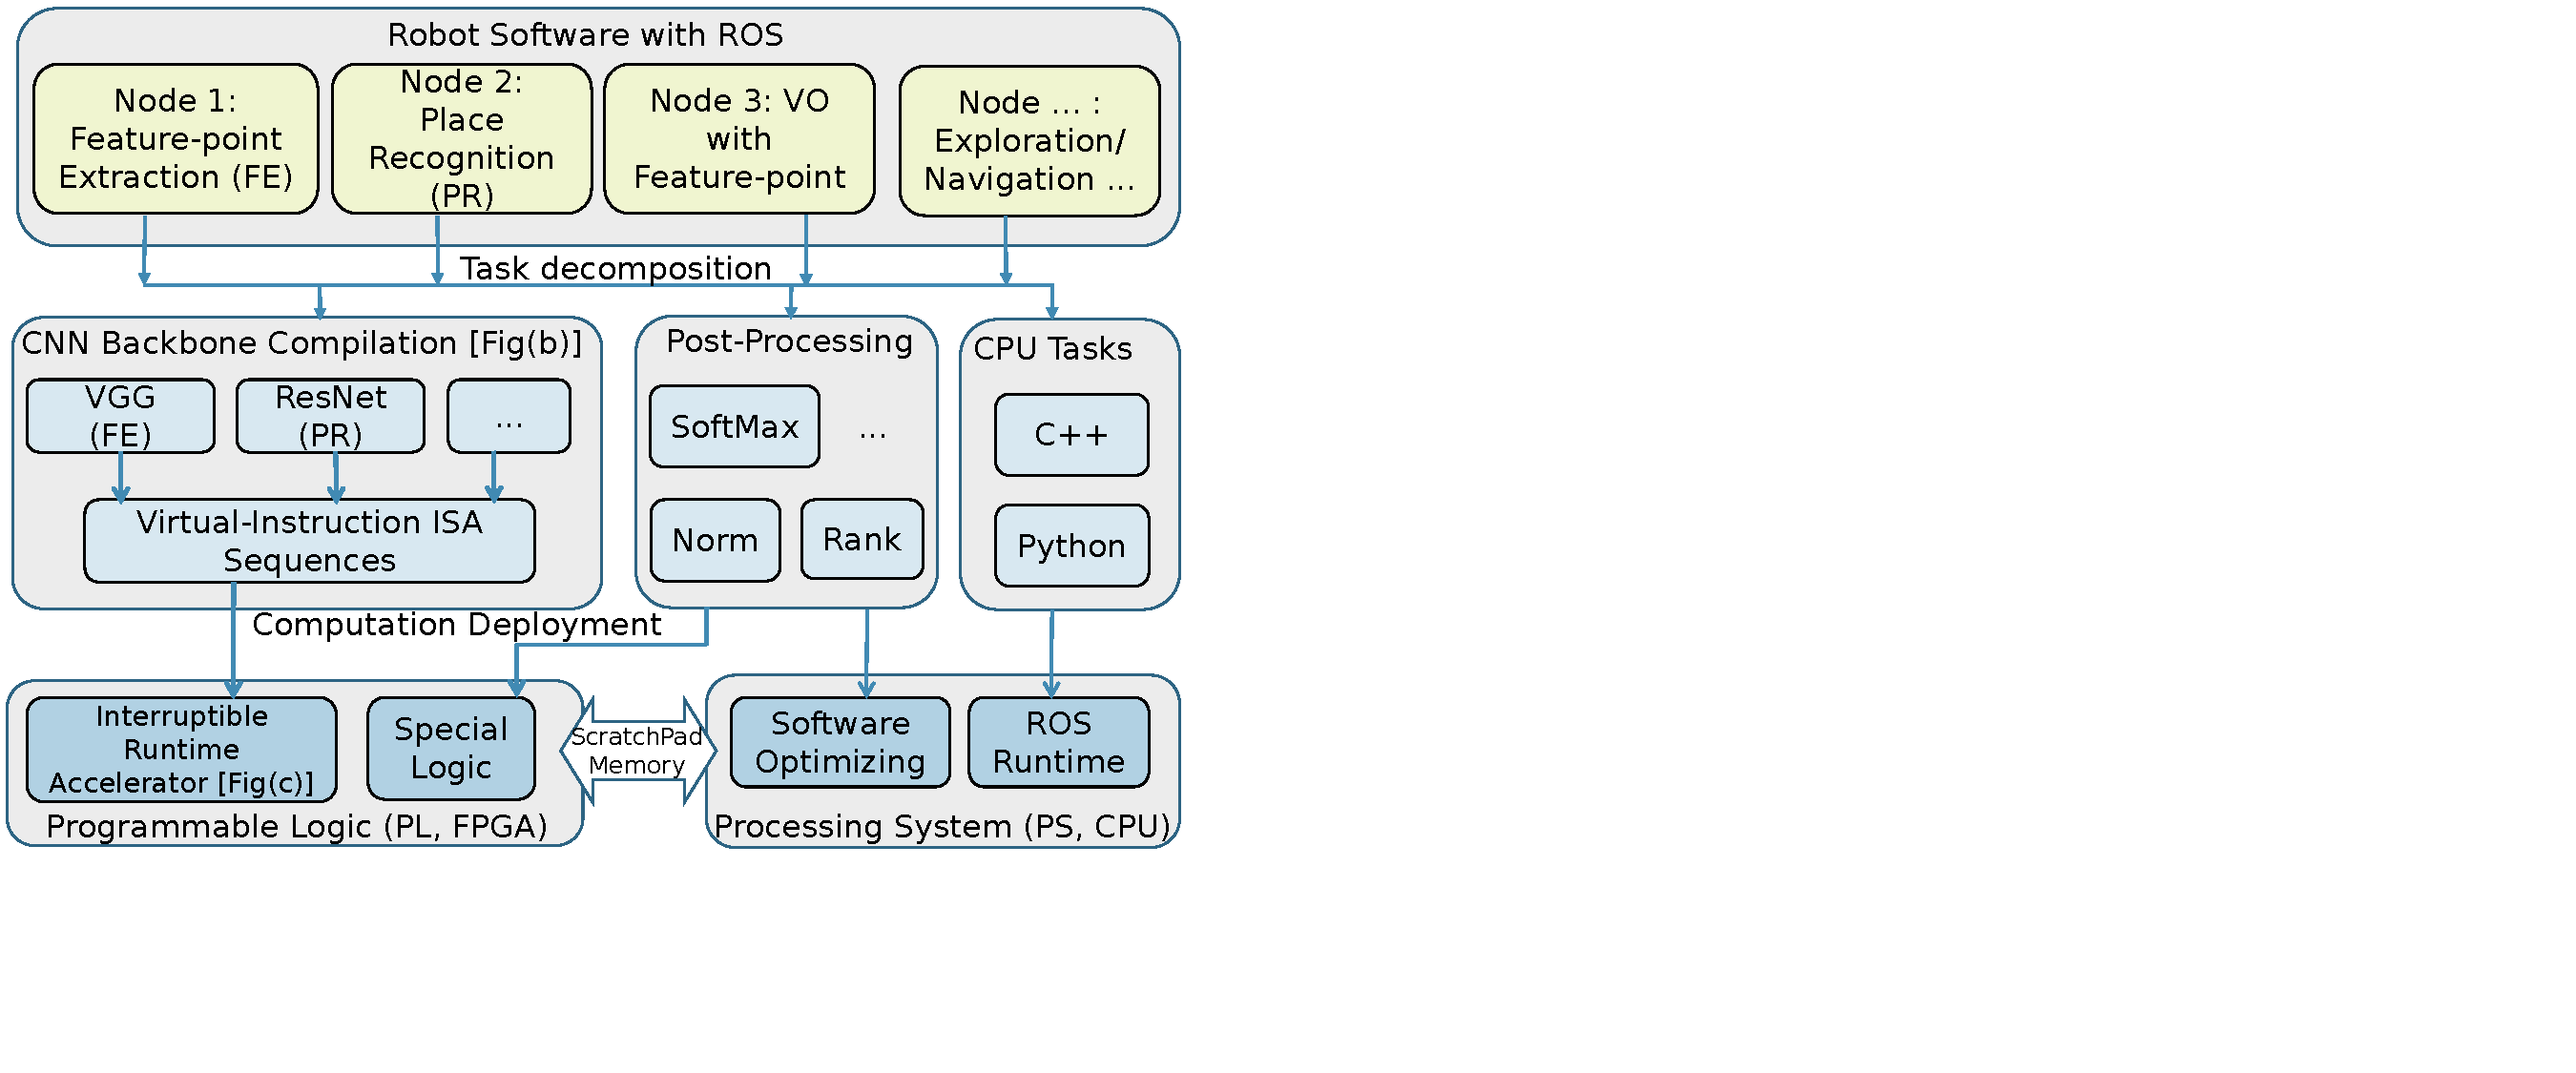
\includegraphics[width=0.99\linewidth]{fig/inca.pdf}
    \caption{ INCA framework. At task decomposition step, the operations in different ROS nodes are separated to CNN backbones, CNN Post-Processing, and Other CPU Tasks. At computation deployment, the CNN backbone and Post-Processing are deployed with hardware modules and software optimizing.  
    }
	\label{fig:inca}
\end{figure}

In order to facilitate robotic researchers to run different CNN tasks simultaneously on the FPGA accelerator, the accelerator should support the following features:

\textbf{Multi-thread:} Because different components in a robot are from different developers, thus, Robot Operating System (ROS)  ~\cite{quigley2009ros} is proposed as a middleware to fuse these independent components, and is widely used by robotic researchers. Each component is considered as an independent thread in ROS. Different threads should have independent access to the accelerator without knowing the status of others.

\textbf{Finishing before deadline:} In a robot, some tasks must be completed within the specified hard deadlines, such as feature-point extraction. The moving robot's perception, including estimation of itself's location and the obstacles' position, is based on the feature-points. If the feature point extraction is not completed before the deadline, the robot can not estimate the surrounding environment, causing collisions or even damage. Those critical tasks with a more stringent headline need to be performed prior to some non-critical tasks ~\cite{RamsauerKLM17}. In DSLAM, the priority of feature-point extraction (FE) is higher than that of place recognition (PR). Because PR is only related to efficiency, yet FE ensures system safety.

To address above challenges, we propose an INterruptible CNN Accelerator (INCA) for rapid deployment of robot application on FPGA. 
The work flow of INCA is illustrated in \Cref{fig:inca}. 
INCA is a two-step framework for mapping software to embedded FPGA. 
The first step is the task decomposition, which decomposes the computation in ROS nodes into different computation types, including CNN backbones, CNN post-processing, and other CPU tasks.
The second step is to deploy the computation onto the FPGA. 
The CNN backbones of different tasks, such as the VGG model  ~\cite{kim2016accurate} in SupoerPoint feature-point extraction  ~\cite{detone2018superpoint} and the ResNet101 model  ~\cite{he2016deep} in GeM place recognition  ~\cite{radenovic2018fine}, are compiled to the interruptible Virtual-Instruction Instruction Set Architecture (VI-ISA), which runs on the CNN accelerator. The VI-ISA is a simple extension of the original ISA, in which the extension method is not limited to a specific original ISA. Thus, the virtual-instruction-based interrupt can be easily applied to various instruction-based CNN accelerators  ~\cite{yu2018instruction,qiu2016going}, such as Angel-Eye ~\cite{guo2017angel} and DPU ~\cite{dpu}.


% The CNN backbones of different tasks, such as the VGG model  ~\cite{kim2016accurate} in SupoerPoint ~\cite{detone2018superpoint} and the ResNet101 model  ~\cite{he2016deep} in GeM  ~\cite{radenovic2018fine}, are compiled to the interruptible Virtual-Instruction Instruction Set Architecture (VI-ISA), which runs on the CNN accelerator.
% The VI-ISA is a simple extension of the original ISA, in which the extension method is not limited to a specific original ISA. Thus, the virtual-instruction-based interrupt can be easily applied to various instruction-based CNN accelerators  ~\cite{yu2018instruction,qiu2016going}, such as Angel-Eye ~\cite{guo2017angel} and DPU ~\cite{dpu}.


In conclusion, INCA facilitate robotic researchers to run different CNN tasks simultaneously on the FPGA with the following contributions:
\begin{itemize}
\item We propose a \textbf{virtual-instruction-based} interrupt method to make the CNN accelerator support dynamic multi-task scheduling by priority. The method solves the hardware resources conflicts when accelerating different CNN tasks on ROS~\cite{quigley2009ros}.
% \item We only needs to modify the instruction fetch module of the CNN accelerator in hardware to support interrupt. Thus, it is easy to be extended to different instruction-driven CNN accelerators.
\item We propose a CNN-based DSLAM system to evaluate INCA. CNN-based methods for feature-point extraction (FE) and place recognition (PR) are accelerated with FPGA on ROS platform. With the help of the unified interface in ROS, these CNN-based methods can be easily used by other developers in different applications.
\end{itemize}
% In terms of perception, CNN has surpassed traditional algorithms in tasks such as object detection \cite{redmon2018yolov3} and scene segmentation \cite{huang2019mask}. 
% In decision-making, CNN also performs well in path planning \cite{chen2017socially} and dynamic obstacle avoidance \cite{kaufmann2018deep}.

